\documentclass{standalone}
\usepackage{tikz}
\usetikzlibrary{patterns, positioning}


\begin{document}
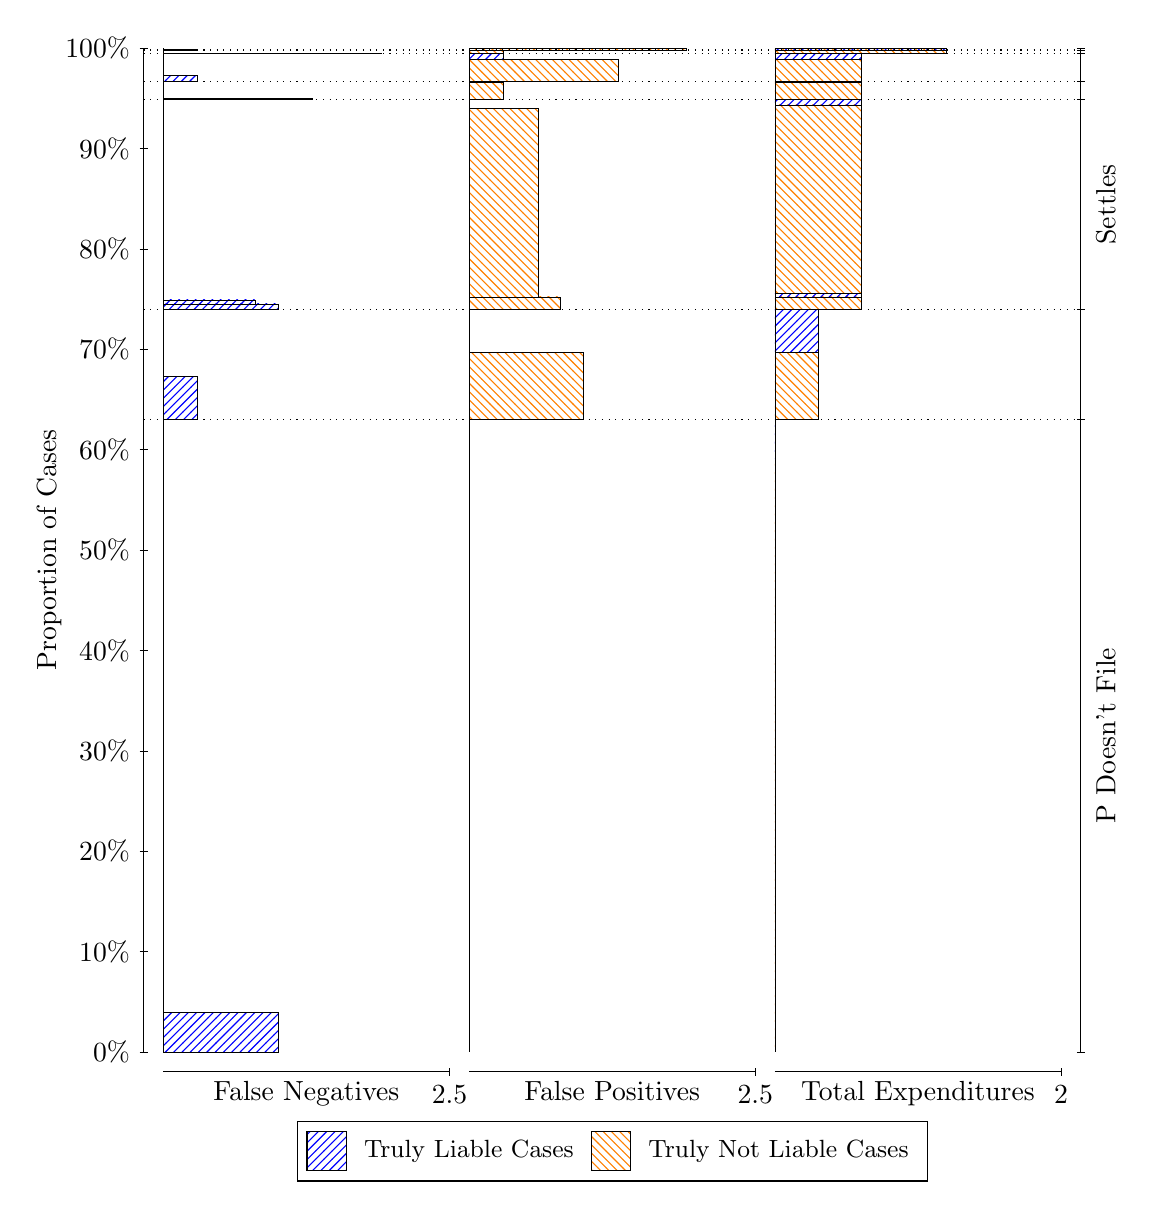
\begin{tikzpicture}
\draw[black, very thin] (1.5,1.75) -- (1.5,14.5);
\node[rotate=90, text=black, anchor=center] at (0.3, 8.125) {Proportion of Cases};
\draw[black, very thin] (1.45,1.75) -- (1.55,1.75);
\node[text=black, anchor=east] at (1.45, 1.75) {0\%};
\draw[black, very thin] (1.45,3.025) -- (1.55,3.025);
\node[text=black, anchor=east] at (1.45, 3.025) {10\%};
\draw[black, very thin] (1.45,4.3) -- (1.55,4.3);
\node[text=black, anchor=east] at (1.45, 4.3) {20\%};
\draw[black, very thin] (1.45,5.575) -- (1.55,5.575);
\node[text=black, anchor=east] at (1.45, 5.575) {30\%};
\draw[black, very thin] (1.45,6.85) -- (1.55,6.85);
\node[text=black, anchor=east] at (1.45, 6.85) {40\%};
\draw[black, very thin] (1.45,8.125) -- (1.55,8.125);
\node[text=black, anchor=east] at (1.45, 8.125) {50\%};
\draw[black, very thin] (1.45,9.4) -- (1.55,9.4);
\node[text=black, anchor=east] at (1.45, 9.4) {60\%};
\draw[black, very thin] (1.45,10.675) -- (1.55,10.675);
\node[text=black, anchor=east] at (1.45, 10.675) {70\%};
\draw[black, very thin] (1.45,11.95) -- (1.55,11.95);
\node[text=black, anchor=east] at (1.45, 11.95) {80\%};
\draw[black, very thin] (1.45,13.225) -- (1.55,13.225);
\node[text=black, anchor=east] at (1.45, 13.225) {90\%};
\draw[black, very thin] (1.45,14.5) -- (1.55,14.5);
\node[text=black, anchor=east] at (1.45, 14.5) {100\%};

\draw[black, very thin] (13.4,1.75) -- (13.4,14.5);
\draw[black, very thin] (13.35,1.75) -- (13.45,1.75);
\node[anchor=west] at (13.35, 1.75) {};
\draw[black, very thin] (13.35,9.7813) -- (13.45,9.7813);
\node[anchor=west] at (13.35, 9.7813) {};
\draw[black, very thin] (13.35,11.181) -- (13.45,11.181);
\node[anchor=west] at (13.35, 11.181) {};
\draw[black, very thin] (13.35,13.849) -- (13.45,13.849);
\node[anchor=west] at (13.35, 13.849) {};
\draw[black, very thin] (13.35,14.078) -- (13.45,14.078);
\node[anchor=west] at (13.35, 14.078) {};
\draw[black, very thin] (13.35,14.429) -- (13.45,14.429);
\node[anchor=west] at (13.35, 14.429) {};
\draw[black, very thin] (13.35,14.475) -- (13.45,14.475);
\node[anchor=west] at (13.35, 14.475) {};
\draw[black, very thin] (13.35,14.5) -- (13.45,14.5);
\node[anchor=west] at (13.35, 14.5) {};

\draw[black, very thin, pattern color=blue, pattern=north east lines] (1.75,1.75) rectangle (3.2033,2.2533);
\draw[black, very thin, pattern color=orange, pattern=north west lines] (1.75,2.2533) rectangle (1.75,9.7813);
\draw[black, very thin, pattern color=blue, pattern=north east lines] (1.75,9.7813) rectangle (2.186,10.332);
\draw[black, very thin, pattern color=orange, pattern=north west lines] (1.75,10.332) rectangle (1.75,11.181);
\draw[black, very thin, pattern color=blue, pattern=north east lines] (1.75,11.181) rectangle (3.2033,11.252);
\draw[black, very thin, pattern color=blue, pattern=north east lines] (1.75,11.252) rectangle (2.9127,11.302);
\draw[black, very thin, pattern color=orange, pattern=north west lines] (1.75,11.302) rectangle (1.75,13.849);
\draw[black, very thin, pattern color=blue, pattern=north east lines] (1.75,13.849) rectangle (3.6393,13.865);
\draw[black, very thin, pattern color=orange, pattern=north west lines] (1.75,13.865) rectangle (1.75,14.078);
\draw[black, very thin, pattern color=blue, pattern=north east lines] (1.75,14.078) rectangle (2.186,14.156);
\draw[black, very thin, pattern color=orange, pattern=north west lines] (1.75,14.156) rectangle (1.75,14.429);
\draw[black, very thin, pattern color=blue, pattern=north east lines] (1.75,14.429) rectangle (4.5113,14.432);
\draw[black, very thin, pattern color=orange, pattern=north west lines] (1.75,14.432) rectangle (1.75,14.475);
\draw[black, very thin, pattern color=blue, pattern=north east lines] (1.75,14.475) rectangle (2.186,14.48);
\draw[black, very thin, pattern color=orange, pattern=north west lines] (1.75,14.48) rectangle (1.75,14.5);
\draw[black, very thin, pattern color=orange, pattern=north west lines] (5.6333,1.75) rectangle (5.6333,9.278);
\draw[black, very thin, pattern color=blue, pattern=north east lines] (5.6333,9.278) rectangle (5.6333,9.7813);
\draw[black, very thin, pattern color=orange, pattern=north west lines] (5.6333,9.7813) rectangle (7.0867,10.63);
\draw[black, very thin, pattern color=blue, pattern=north east lines] (5.6333,10.63) rectangle (5.6333,11.181);
\draw[black, very thin, pattern color=orange, pattern=north west lines] (5.6333,11.181) rectangle (6.796,11.339);
\draw[black, very thin, pattern color=orange, pattern=north west lines] (5.6333,11.339) rectangle (6.5053,13.729);
\draw[black, very thin, pattern color=blue, pattern=north east lines] (5.6333,13.729) rectangle (5.6333,13.849);
\draw[black, very thin, pattern color=orange, pattern=north west lines] (5.6333,13.849) rectangle (6.0693,14.062);
\draw[black, very thin, pattern color=blue, pattern=north east lines] (5.6333,14.062) rectangle (5.6333,14.078);
\draw[black, very thin, pattern color=orange, pattern=north west lines] (5.6333,14.078) rectangle (7.5227,14.351);
\draw[black, very thin, pattern color=blue, pattern=north east lines] (5.6333,14.351) rectangle (6.0693,14.429);
\draw[black, very thin, pattern color=orange, pattern=north west lines] (5.6333,14.429) rectangle (6.0693,14.473);
\draw[black, very thin, pattern color=blue, pattern=north east lines] (5.6333,14.473) rectangle (5.6333,14.475);
\draw[black, very thin, pattern color=orange, pattern=north west lines] (5.6333,14.475) rectangle (8.3947,14.496);
\draw[black, very thin, pattern color=blue, pattern=north east lines] (5.6333,14.496) rectangle (6.9413,14.5);
\draw[black, very thin, pattern color=orange, pattern=north west lines] (9.5167,1.75) rectangle (9.5167,9.278);
\draw[black, very thin, pattern color=blue, pattern=north east lines] (9.5167,9.278) rectangle (9.5167,9.7813);
\draw[black, very thin, pattern color=orange, pattern=north west lines] (9.5167,9.7813) rectangle (10.062,10.63);
\draw[black, very thin, pattern color=blue, pattern=north east lines] (9.5167,10.63) rectangle (10.062,11.181);
\draw[black, very thin, pattern color=orange, pattern=north west lines] (9.5167,11.181) rectangle (10.607,11.339);
\draw[black, very thin, pattern color=blue, pattern=north east lines] (9.5167,11.339) rectangle (10.607,11.388);
\draw[black, very thin, pattern color=orange, pattern=north west lines] (9.5167,11.388) rectangle (10.607,13.778);
\draw[black, very thin, pattern color=blue, pattern=north east lines] (9.5167,13.778) rectangle (10.607,13.849);
\draw[black, very thin, pattern color=orange, pattern=north west lines] (9.5167,13.849) rectangle (10.607,14.062);
\draw[black, very thin, pattern color=blue, pattern=north east lines] (9.5167,14.062) rectangle (10.607,14.078);
\draw[black, very thin, pattern color=orange, pattern=north west lines] (9.5167,14.078) rectangle (10.607,14.351);
\draw[black, very thin, pattern color=blue, pattern=north east lines] (9.5167,14.351) rectangle (10.607,14.429);
\draw[black, very thin, pattern color=orange, pattern=north west lines] (9.5167,14.429) rectangle (11.697,14.473);
\draw[black, very thin, pattern color=blue, pattern=north east lines] (9.5167,14.473) rectangle (11.697,14.475);
\draw[black, very thin, pattern color=orange, pattern=north west lines] (9.5167,14.475) rectangle (11.697,14.496);
\draw[black, very thin, pattern color=blue, pattern=north east lines] (9.5167,14.496) rectangle (11.697,14.5);
\draw[black, dotted] (1.5,9.7813) -- (13.4,9.7813);
\draw[black, dotted] (1.5,11.181) -- (13.4,11.181);
\draw[black, dotted] (1.5,13.849) -- (13.4,13.849);
\draw[black, dotted] (1.5,14.078) -- (13.4,14.078);
\draw[black, dotted] (1.5,14.429) -- (13.4,14.429);
\draw[black, dotted] (1.5,14.475) -- (13.4,14.475);
\draw[black, very thin] (1.75,1.5) -- (5.3833,1.5);
\node[text=black, anchor=north] at (3.5667, 1.5) {False Negatives};
\draw[black, very thin] (5.3833,1.45) -- (5.3833,1.55);
\node[text=black, anchor=north] at (5.3833, 1.45) {2.5};

\draw[black, very thin] (5.6333,1.5) -- (9.2667,1.5);
\node[text=black, anchor=north] at (7.45, 1.5) {False Positives};
\draw[black, very thin] (9.2667,1.45) -- (9.2667,1.55);
\node[text=black, anchor=north] at (9.2667, 1.45) {2.5};

\draw[black, very thin] (9.5167,1.5) -- (13.15,1.5);
\node[text=black, anchor=north] at (11.333, 1.5) {Total Expenditures};
\draw[black, very thin] (13.15,1.45) -- (13.15,1.55);
\node[text=black, anchor=north] at (13.15, 1.45) {2};

\node[text=black, centered, rotate=90] at (13.72, 5.7656) {P Doesn't File};

\node[text=black, centered, rotate=90] at (13.72, 12.515) {Settles};





\draw (7.449999999999999,1.5) node[draw=none] (baseCoordinate) {};
\begin{scope}[align=center]
        \matrix[scale=0.5, draw=black, below=0.5cm of baseCoordinate, nodes={draw}, column sep=0.1cm]{
            \node[rectangle, draw, minimum width=0.5cm, minimum height=0.5cm, pattern color=blue, pattern=north east lines] {}; &
            \node[draw=none, font=\small, text=black] (B) {Truly Liable Cases}; &
            \node[rectangle, draw, minimum width=0.5cm, minimum height=0.5cm, pattern color=orange, pattern=north west lines] {}; &
            \node[draw=none, font=\small, text=black] (B) {Truly Not Liable Cases}; \\
            };
\end{scope}

\end{tikzpicture}
\end{document}